\documentclass[main.tex]{subfiles}
%% Current Author: PS
\setcounter{chapter}{13}
\begin{document}
\chapter{Electromagnetism}
\spec{understand and use the terms magnetic flux density, flux and flux linkage}

Electromagnetic induction depends crucially on the concept of \emph{flux}. This is the product of the magnetic field strength $B$ and the area of a loop perpendicular to the field, $A$.
\[ \Phi = BA \]
The unit of flux is the weber, Wb. Given its relation to flux, the field strength $B$ can also be referred to as the magnetic flux density. It also follows that the tesla is equivalent to one weber per metre-squared.

When a coil of wire encloses an area of flux we can calculate the \emph{flux-linkage} which is the product of the flux through the coil and the number of turns on the coil, $N\Phi$.

\spec{understand that magnetic fields are created by electric current}

An electric current in a wire creates a magnetic field. The field strength depends on the size of the current and the distance from the wire. In the case of a solenoid or electromagnet the field strength is also proportional to the number of turns on the coil.

\spec{recognise and use  $F = BIl\sin\theta$}

This is the equation for the force on a current-carrying wire of length $l$ with a current of $I$ at an angle $\theta$ to a magnetic field of strength $B$.

\spec{recognise and use $F = BQv\sin\theta$}

This is the equation for a particle of charge $Q$ moving at a velocity $v$ at an angle $\theta$ to a magnetic field of strength $B$. Note that this is sometimes called the Lorentz force.

\spec{use Fleming's left-hand rule to solve problems}

Fleming's left-hand rule allows the calculation of the direction of the force on either a charged particle or a current-carrying wire. The geometry is shown below.

\begin{figure}[h]
  \begin{center}
  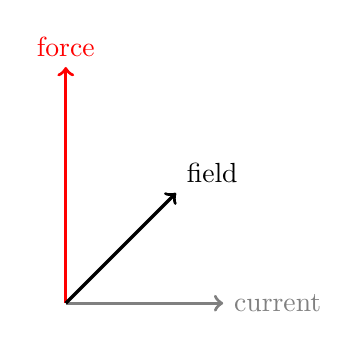
\begin{tikzpicture}
      \draw [->, gray,very thick] (0,0) -- (2,0) node[anchor=west] {current};
      \draw [->, red,very thick] (0,0) -- (0,3) node[anchor=south] {force};
      \draw [->, black,very thick] (0,0) -- (1.4,1.4) node[anchor=south west] {field};
    \end{tikzpicture}
  \end{center}
  \caption{Fleming's left-hand rule}
  \label{flemminglh}
\end{figure}

\spec{explain qualitatively the factors affecting the emf induced across a coil when there is relative motion between the coil and a permanent magnet or when there is a change of current in a primary coil linked with it}

Since the emf depends on the rate of change of flux linkage the size of the emf is proportional to the number of turns on a coil. The rate of change of flux is determined by strength of the magnet and how quickly it is moving through the coil.

\spec{recognise and use $E=-\frac{d(N\Phi)}{dt}$ and explain how it is an expression of Faraday’s and Lenz’s laws}

Since $N\Phi$ is the flux linkage then $\frac{d(N\Phi)}{dt}$ is the rate of change of flux linkage. The negative sign indicates that the induced emf acts to oppose the change in flux linkage which created it (which is Lenz's Law).

\spec{derive, recall and use $r = \frac{mv}{BQ}$ for the radius of curvature of a deflected charged particle}

When a charged particle moves through a uniform magnetic field at a constant speed it experiences a constant force at right-angles to its velocity. This results in it moving in circular motion with the Lorentz force providing the centripetal force.
\[ BQv = \frac{mv^2}{r} \]
\[\implies r = \frac{mv}{BQ} \]

This allows the calculation of the mass to charge ratio of the particle providing its velocity can be determined (e.g. from an accelerating potential).

\spec{explain the Hall effect, and derive and use $V = Bvd$}

When an electron moves through a magnetic field it will experience a force at right-angles to its motion. If a current flows through a thin film of material then a negative charge will accumulate on one edge of the film. Figure \ref{halleffect} shows this force acting and charge building up.

\begin{figure}[h]
  \begin{center}
  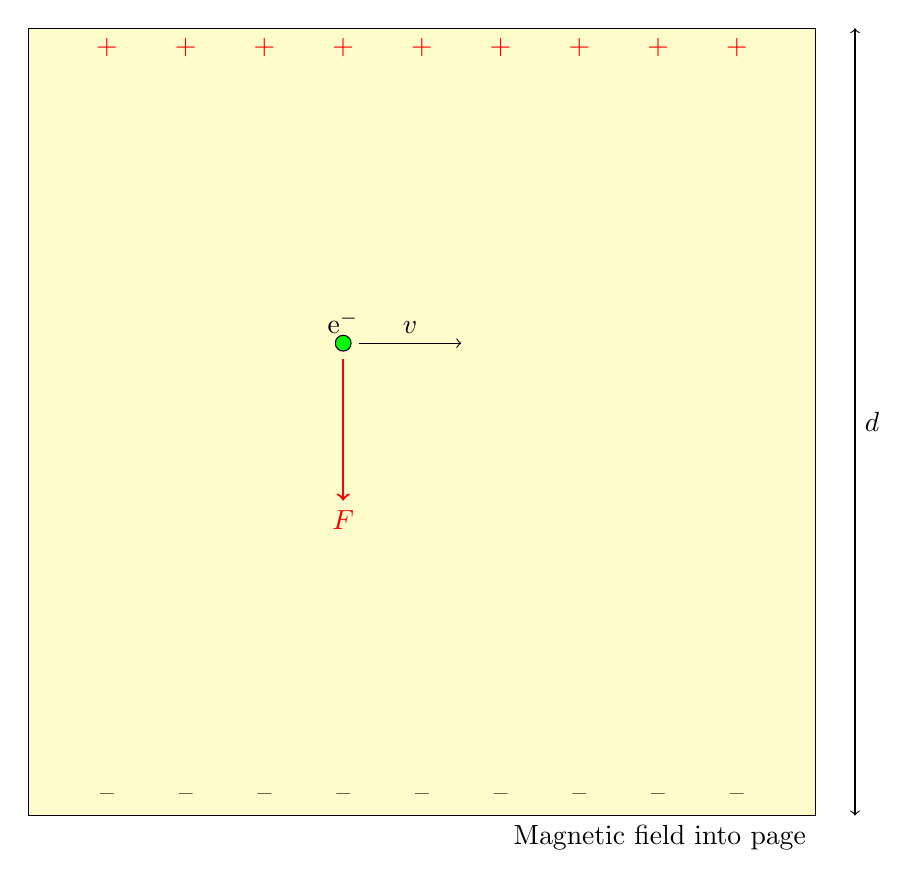
\begin{tikzpicture}
    \filldraw [fill=yellow!20!white,draw=black] (0,0) rectangle (10,10);
    \draw (10,0)  node[anchor=north east] {Magnetic field into page};
    \filldraw[fill=green] (4,6) circle (0.1) node[anchor=south] {e$^-$};
    \draw[->] (4.2,6) -- (5.5,6) node[midway,above]{$v$};
    \draw[->, thick, red] (4,5.8) -- (4,4) node[anchor=north] {$F$};
    \foreach \x in {1,2,...,9} 
        {\draw (\x,.25) node{--};\draw[color=red] (\x,9.75) node{+};}
    \draw[<->] (10.5,0) -- (10.5,10) node[midway, right] {$d$};
  \end{tikzpicture}
  \end{center}
  \caption{The Hall Effect}
  \label{halleffect}
\end{figure}

Over time the charges build up on either side of the wager until equilibrium is reached. At this point the the force due to the electric field on the charge equals the force due to the Lorentz force on the charge.
$$ q\frac{V}{d} = Bqv $$
$$ V_\text{hall} = Bvd $$

This relationship is the basis of a Hall Probe which is used to measure magnetic fields. In these circumstances the velocity $v$ is the drift velocity of the electrons.


\end{document}

%sagemathcloud={"latex_command":"latexmk -xelatex -f -g -bibtex -synctex=1 -interaction=nonstopmode '14-electromagnetism.tex'"}